%%% Copyright (C) 2017 Vincent Goulet, David Beauchemin, Samuel Cabral Cruz
%%%
%%% Ce fichier et tous les fichiers .tex ou .Rnw dont la racine est
%%% mentionnée dans les commandes \include ci-dessous font partie du
%%% projet «Introduction à R - Atelier du colloque R à Québec 2017»
%%% http://github.com/vigou3/raquebec-atelier-introduction-r
%%%
%%% Cette création est mise à disposition selon le contrat
%%% Attribution-Partage dans les mêmes conditions 4.0
%%% International de Creative Commons.
%%% http://creativecommons.org/licenses/by-sa/4.0/

\documentclass[aspectratio=1610,10pt,xcolor=x11names]{beamer}
  \usepackage[french]{babel}
  \usepackage[autolanguage]{numprint}
  \usepackage[noae]{Sweave}
  \usepackage{fontawesome}
  \usepackage{changepage}                % page licence
  \usepackage{tabularx}                  % page licence
  \usepackage{listings}                  % code source
  \usepackage{framed}                    % env. leftbar
  \usepackage[export]{adjustbox}         % cadre autour image
  \usepackage[overlay,absolute]{textpos} % couvertures
  \usepackage{metalogo}                  % logo \XeLaTeX

  %% =============================
  %%  Informations de publication
  %% =============================
  \renewcommand{\year}{2017}
  \renewcommand{\month}{5}

  %% =======================
  %%  Apparence du document
  %% =======================

  %% Thème de beamer
  \usetheme{metropolis}

  %% Couleurs additionnelles
  \definecolor{comments}{rgb}{0.7,0,0}      % commentaires
  \definecolor{link}{rgb}{0,0.4,0.6}        % liens internes
  \definecolor{url}{rgb}{0.6,0,0}           % liens externes
  \definecolor{codebg}{named}{LightYellow1} % fond code R
  \definecolor{rouge}{rgb}{0.85,0,0.07}     % rouge bandeau identitaire
  \definecolor{or}{rgb}{1,0.8,0}            % or bandeau identitaire

  %% Hyperliens
  \hypersetup{%
    pdfauthor = {David Beauchemin, Samuel Cabral Cruz, Vincent Goulet},
    pdftitle = {Atelier Introduction à R du colloque R à Québec},
    colorlinks = {true},
    linktocpage = {true},
    allcolors = {link},
    urlcolor = {url},
    pdfpagemode = {UseOutlines},
    pdfstartview = {Fit},
    bookmarksopen = {true},
    bookmarksnumbered = {true},
    bookmarksdepth = {subsection}}

  %% Paramétrage de babel pour les guillemets
  \frenchbsetup{og=«, fg=»}

  %% Sections de code source
  \lstloadlanguages{R}
  \lstset{language=R,
    extendedchars=true,
    basicstyle=\small\ttfamily\NoAutoSpacing,
    commentstyle=\color{comments}\slshape,
    keywordstyle=\mdseries,
    escapeinside=`',
    aboveskip=0pt,
    belowskip=0pt,
    showstringspaces=false}

  %% =========================
  %%  Nouveaux environnements
  %% =========================

  %% Environnements de Sweave.
  %%
  %% Les environnements Sinput et Soutput utilisent Verbatim (de
  %% fancyvrb). On les réinitialise pour enlever la configuration par
  %% défaut de Sweave, puis on réduit l'écart entre les blocs Sinput
  %% et Soutput.
  \DefineVerbatimEnvironment{Sinput}{Verbatim}{}
  \DefineVerbatimEnvironment{Soutput}{Verbatim}{}
  \fvset{fontsize=\small,listparameters={\setlength{\topsep}{0pt}}}

  %% L'environnement Schunk est complètement redéfini en un hybride
  %% des environnements snugshade* et leftbar de framed.
  \makeatletter
  \renewenvironment{Schunk}{%
    \def\FrameCommand##1{\hskip\@totalleftmargin
      \vrule width 3pt\colorbox{codebg}{\hspace{5pt}##1}%
      % There is no \@totalrightmargin, so:
      \hskip-\linewidth \hskip-\@totalleftmargin \hskip\columnwidth}%
    \MakeFramed {\advance\hsize-\width
      \@totalleftmargin\z@ \linewidth\hsize
      \advance\labelsep\fboxsep
      \@setminipage}%
  }{\par\unskip\@minipagefalse\endMakeFramed}
  \makeatother

  %% =====================
  %%  Nouvelles commandes
  %% =====================

  %% Noms de fonctions, code, environnement, etc.
  \newcommand{\fichier}[1]{\fbox{\texttt{#1}}}
  \newcommand{\class}[1]{\textbf{#1}}
  \newcommand{\pkg}[1]{\textbf{#1}}
  \newcommand{\link}[2]{\href{#1}{#2~\raisebox{-0.2ex}{\faExternalLink}}}
  \newcommand{\capsule}[2]{\href{#1}{\faYoutubePlay~#2}}

  \newcommand{\meta}[1]{\ensuremath\langle{\normalfont\itshape #1\/}\ensuremath\rangle}

  %% Renvoi vers GitHub sur la page de copyright
  \newcommand{\viewsource}[1]{%
    \href{#1}{%
      \makebox[2.5mm]{\raisebox{-1pt}{\footnotesize\faGithub}}\;%
      {\sffamily Voir sur GitHub}}}

  %% Renvois vers les scripts R
  \newcommand{\gotoR}[1]{%
    \begin{center}
      \colorbox{mDarkTeal}{\color{white}
      \makebox[40mm][c]{%
        \makebox[5mm]{\raisebox{-1pt}{\large\faChevronCircleDown}}\;%
        {\ttfamily #1}}}
    \end{center}}

  %% Renvois vers vidéos YouTube
  \newcommand{\video}[2]{%
    \begin{center}
      \href{#1}{%
        \makebox[5mm]{\raisebox{-2pt}{\Large\faYoutubePlay}}\;{#2}}
    \end{center}}

  %%% =======
  %%%  Varia
  %%% =======

  %% Longueurs pour la composition des pages couvertures avant et
  %% arrière.
  \newlength{\banderougewidth} \newlength{\banderougeheight}
  \newlength{\bandeorwidth}    \newlength{\bandeorheight}
  \newlength{\imageheight}     \newlength{\imagewidth}
  \newlength{\logoheight}
  \newlength{\gapwidth}

  %\includeonly{couverture-avant}

\begin{document}

%% frontmatter
\begingroup

\TPGrid{3}{36}
\textblockorigin{0mm}{0mm}
\setlength{\parindent}{0mm}
\setlength{\banderougewidth}{2\TPHorizModule}
\setlength{\banderougeheight}{\TPVertModule}
\setlength{\bandeorwidth}{\TPHorizModule}
\setlength{\bandeorheight}{\banderougeheight}
\setlength{\imageheight}{29\TPVertModule}
\setlength{\imagewidth}{3\TPHorizModule}
\setlength{\logoheight}{2.5\TPVertModule}
\setlength{\gapwidth}{0.75pt}
\addtolength{\bandeorwidth}{-\gapwidth}
\addtolength{\imageheight}{-\gapwidth}

\begin{frame}[plain]
  %% bandeau identitaire
  \begin{textblock*}{3\TPHorizModule}[0,1](0mm,30\TPVertModule)
    \textcolor{rouge}{\rule{\banderougewidth}{\banderougeheight}}% % bande rouge
    \rule{\gapwidth}{0pt}%                                         % filet
    \textcolor{or}{\rule{\bandeorwidth}{\bandeorheight}}           % bande or
  \end{textblock*}

  %% logo UL
  \begin{textblock*}{\TPHorizModule}(2\TPHorizModule,31\TPVertModule)
    \rule{\gapwidth}{0pt}%                                     % filet
    \includegraphics[height=\logoheight,keepaspectratio=true]{ul_p}
  \end{textblock*}

  %% image de fond
  \begin{textblock*}{3\TPHorizModule}(0mm,0mm)
    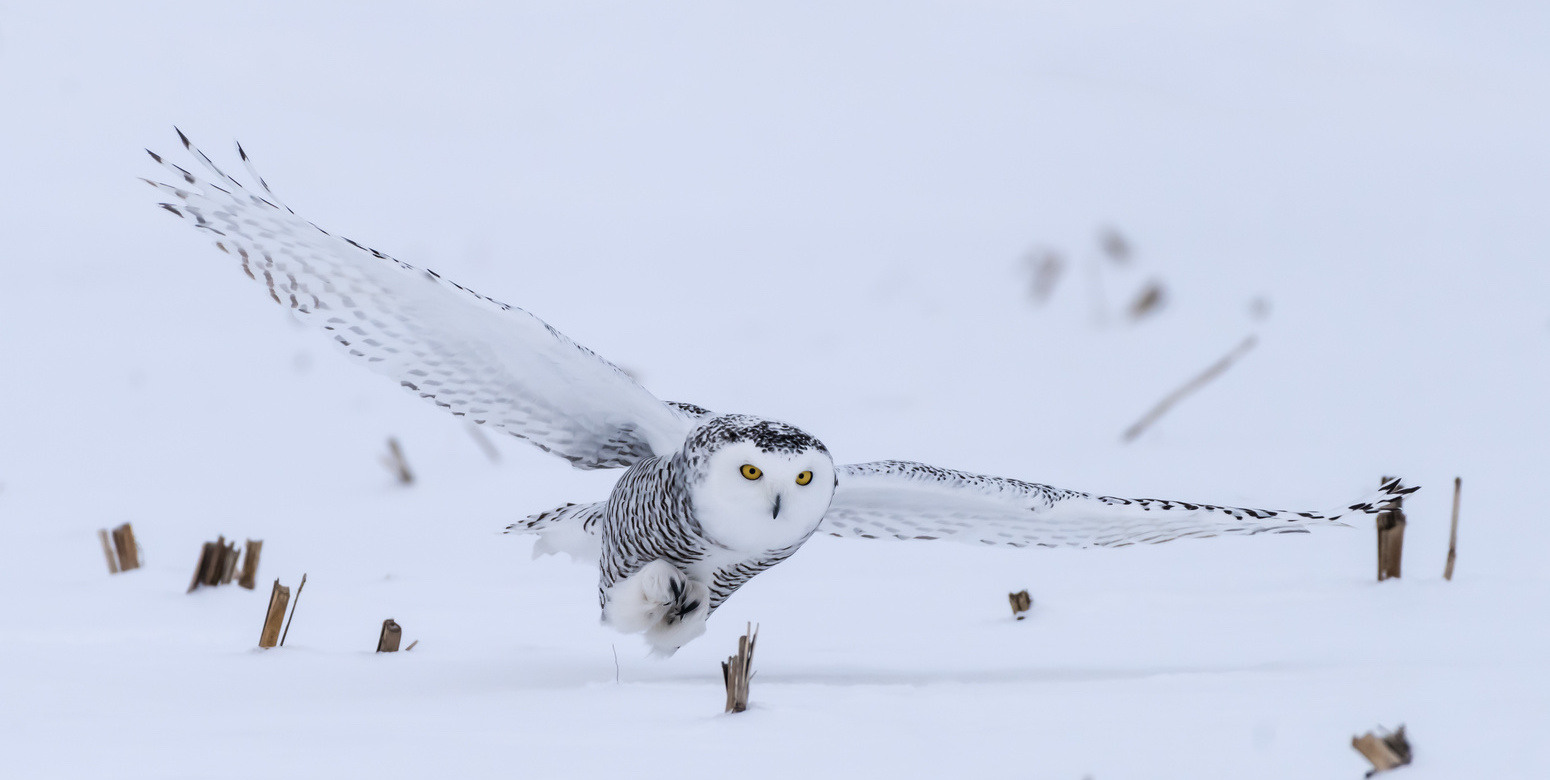
\includegraphics[height=\imageheight,width=\imagewidth]{Fotolia_99831160.jpg}
  \end{textblock*}

  %% titre
  \begin{textblock*}{2\TPHorizModule}(0.2\TPHorizModule,3\TPVertModule)
    \raggedright%
    \bfseries
    \fontsize{30}{30}\selectfont
    Introduction à R \\
    \mdseries
    \fontsize{14}{18}\selectfont
    Atelier du colloque R à Québec 2017
  \end{textblock*}

  %% date
  \begin{textblock*}{2\TPHorizModule}(0.2\TPHorizModule,26\TPVertModule)
    \fontsize{10}{12}\selectfont
    25 mai 2017
  \end{textblock*}
\end{frame}
\endgroup

%%% Local Variables:
%%% mode: latex
%%% TeX-engine: xetex
%%% TeX-master: "raquebec-atelier-introduction-r"
%%% End:

\begingroup

\TPGrid{3}{36}
\textblockorigin{0mm}{0mm}
\begin{frame}[plain]
  %% titre
  \begin{textblock*}{2\TPHorizModule}(0.2\TPHorizModule,3\TPVertModule)
    \raggedright%
    \bfseries
    \fontsize{30}{30}\selectfont
    Introduction à R \\
    \mdseries
    \fontsize{14}{18}\selectfont
    Atelier du colloque R à Québec 2017 \\
  \end{textblock*}

  %% auteurs
  \begin{textblock*}{2\TPHorizModule}(0.2\TPHorizModule,15\TPVertModule)
    \fontsize{10}{11}\selectfont
    \bfseries
    Vincent Goulet \\
    \fontsize{9}{11}\selectfont
    \mdseries
    Professeur titulaire | École d'actuariat \\[6pt]
    \fontsize{10}{11}\selectfont
    \bfseries
    David Beauchemin \\
    \fontsize{9}{11}\selectfont
    \mdseries
    École d'actuariat \\[6pt]
    \fontsize{10}{11}\selectfont
    \bfseries
    Samuel Cabral Cruz \\
    \fontsize{9}{11}\selectfont
    \mdseries
    Desjardins Assurances Générales
  \end{textblock*}
\end{frame}
\endgroup

%%% Local Variables:
%%% mode: latex
%%% TeX-engine: xetex
%%% TeX-master: "raquebec-atelier-introduction-r"
%%% End:

%%% Texte du contrat de licence au début des diapos

\begin{frame}[t,plain,fragile=singleslide]
  \tiny
  \vspace*{10mm}

  \begin{adjustwidth}{15mm}{15mm}
    {\textcopyright} {\year} Vincent Goulet, David Beauchemin, Samuel
    Cabral Cruz \\[4mm]

    
\includegraphics[height=4mm,keepaspectratio=true]{by-sa} \\%

    Cette création est mise à disposition selon le contrat
    \href{http://creativecommons.org/licenses/by-sa/4.0/deed.fr}{%
      Attribution-Partage dans les mêmes conditions 4.0 International}
    de Creative Commons. En vertu de ce contrat, vous êtes libre de:
    \begin{itemize}
    \item \textbf{partager} --- reproduire, distribuer et communiquer
      l'{\oe}uvre;
    \item \textbf{remixer} --- adapter l'{\oe}uvre;
    \item utiliser cette {\oe}uvre à des fins commerciales.
    \end{itemize}
    Selon les conditions suivantes: \vspace*{2mm}

    \begin{tabularx}{\linewidth}{@{}lX@{}}
      \raisebox{-5.5mm}[0mm][10mm]{%
      
\includegraphics[height=7mm,keepaspectratio=true]{by}} &
      \textbf{Attribution} --- Vous devez créditer l'{\oe}uvre, intégrer
      un lien vers le contrat et indiquer si des modifications ont été
      effectuées à l'{\oe}uvre. Vous devez indiquer ces informations par
      tous les moyens possibles, mais vous ne pouvez suggérer que
      l'Offrant vous soutient ou soutient la façon dont vous avez
      utilisé son {\oe}uvre. \\
      \raisebox{-5.5mm}{
\includegraphics[height=7mm,keepaspectratio=true]{sa}}
      & \textbf{Partage dans les mêmes conditions} --- Dans le cas où
      vous modifiez, transformez ou créez à partir du matériel composant
      l'{\oe}uvre originale, vous devez diffuser l'{\oe}uvre modifiée
      dans les même conditions, c'est à dire avec le même contrat avec
      lequel l'{\oe}uvre originale a été diffusée.
    \end{tabularx}
    \vspace{5mm}

    \textbf{Code source} \\
    \viewsource{https://github.com/vigou3/raquebec-intro/}
  \end{adjustwidth}
\end{frame}

%%% Local Variables:
%%% mode: latex
%%% TeX-engine: xetex
%%% TeX-master: "raquebec-atelier-introduction-r"
%%% End:

\begin{frame}
  \frametitle{Référence pour la formation}

  \begin{columns}
    \begin{column}{.5\textwidth}
      Goulet V., avec la colloboration de
      Laurent Caron. 2016. \\
      \emph{Introduction à la programmation en R},
      cinquième édition révisée. \\
      Document libre sous contrat Creative
      Commons. \\
      ISBN 978-2-9811416-6-8.
      \bigskip

      \href{https://vigou3.github.io/introduction-programmation-r}{%
        Consulter la page du projet}
    \end{column}
    \begin{column}{.4\textwidth}
      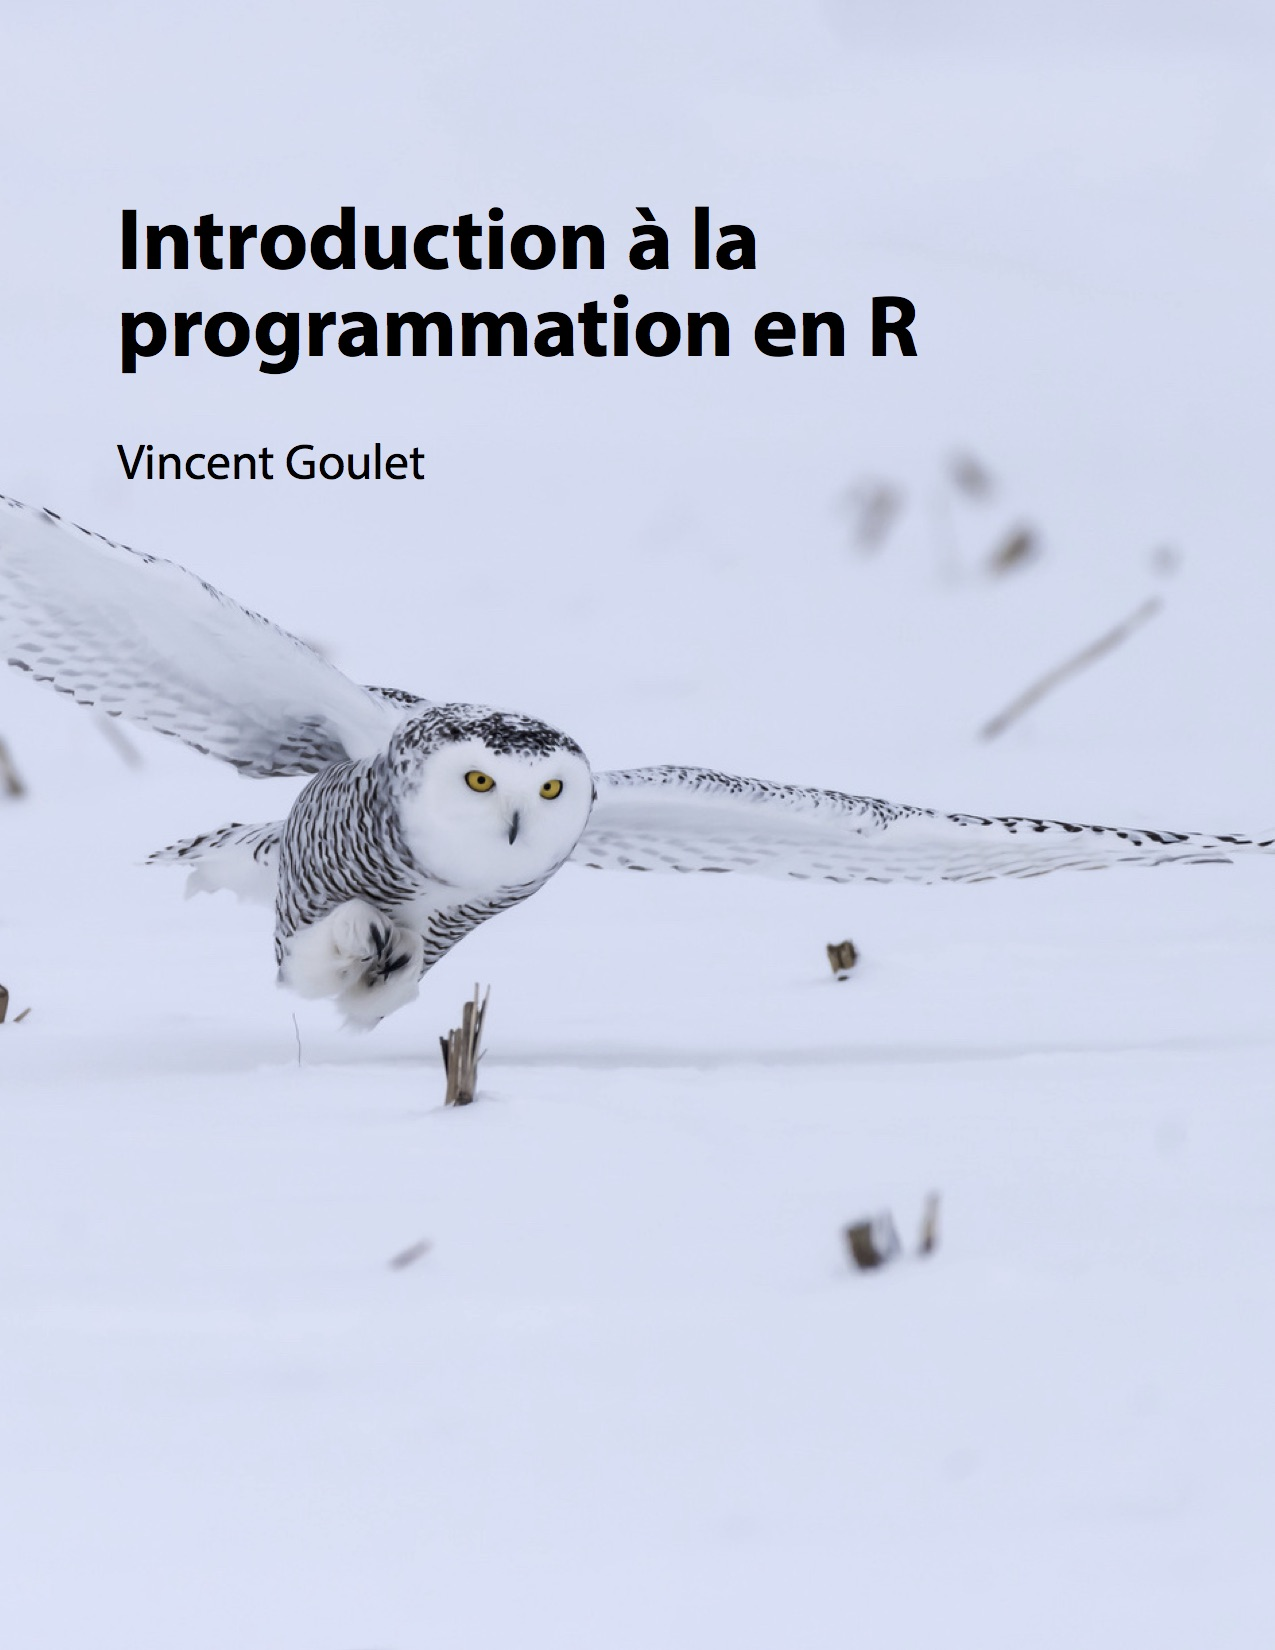
\includegraphics[width=\linewidth,frame]{introduction-programmation-r}
    \end{column}
  \end{columns}
\end{frame}

%%% Local Variables:
%%% mode: latex
%%% TeX-engine: xetex
%%% TeX-master: "raquebec-atelier-introduction-r"
%%% End:


%% mainmatter
\section{Présentation de R}

\begin{frame}
  \frametitle{Bref historique}

  «\emph{R is a free software environment for statistical computing and graphics}»
  \bigskip

  \begin{itemize}
  \item À l'origine fut le S --- milieu des années 1970 --- John~M.\ Chambers
  \item Principalement popularisé par mise en {\oe}uvre commerciale
    S-PLUS
  \end{itemize}
  \bigskip

  \begin{quote}
    \begin{minipage}{0.35\linewidth}
      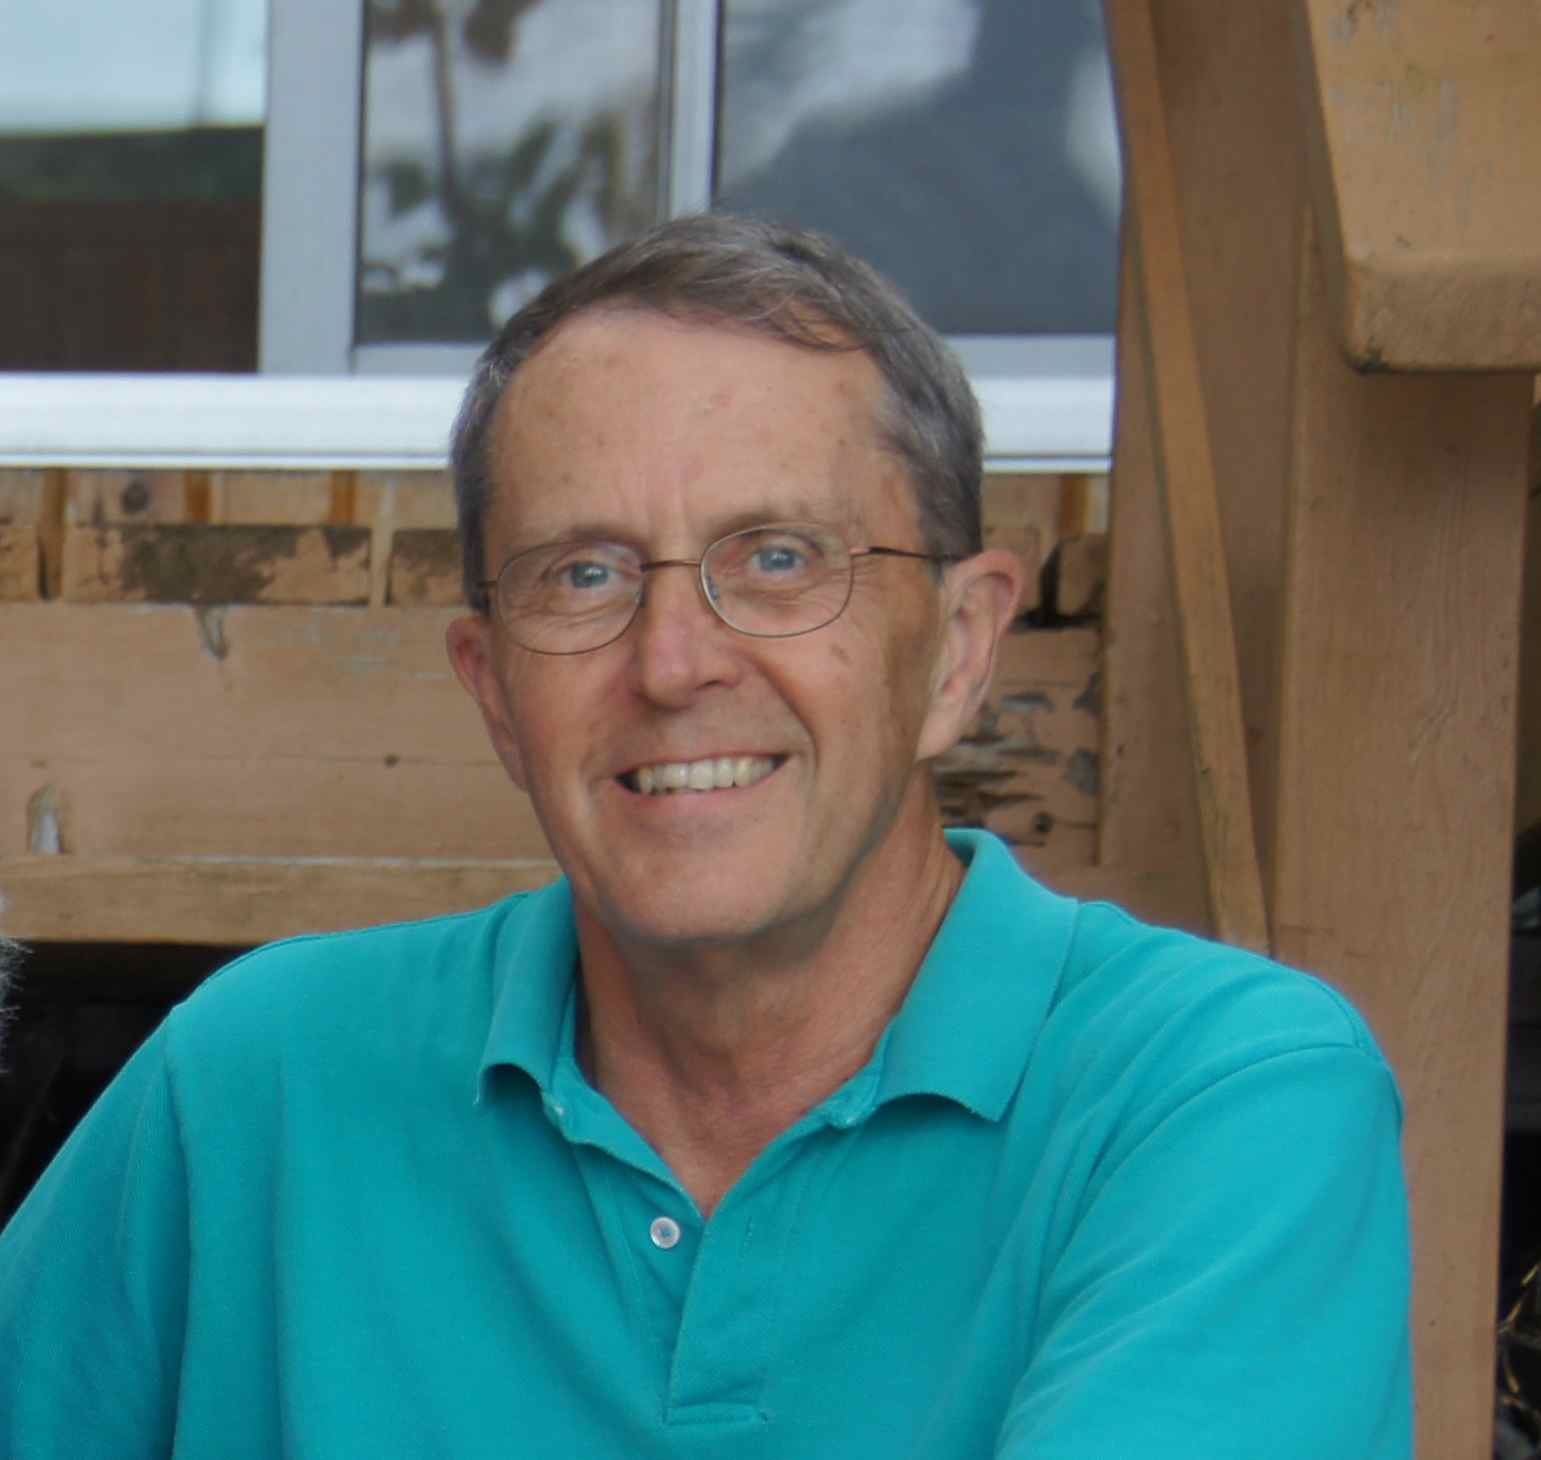
\includegraphics[width=\linewidth,keepaspectratio]{Chambers}
    \end{minipage}
    \hfill
    \begin{minipage}{0.6\linewidth}
      \raggedright
      \textbf{ACM Software System Award 1998} \\
      \emph{John Chambers --- Langage S} \\[\baselineskip]

      «\dots\ which has forever altered how people analyse,
        visualize and manipulate data»
    \end{minipage}
  \end{quote}
\end{frame}

\begin{frame}[fragile=singleslide]
  \frametitle{Bref historique (suite)}

  \begin{itemize}
  \item Nouvelle mise en {\oe}uvre du langage --- milieu des années
    1990 --- \textbf{R}oss Ihaka et \textbf{R}obert Gentleman
  \item Inspirée de Scheme (un dérivé du Lisp) avec syntaxe du S
\begin{Schunk}
\begin{Sinput}
(define factorial (lambda (n)
  (if (= n 1)
      1
    (* n (factorial (- n 1))))))
\end{Sinput}
\end{Schunk}
vs
\begin{Schunk}
\begin{Sinput}
factorial <- function(n)
  if (n == 1) 1 else n * factorial(n - 1)
\end{Sinput}
\end{Schunk}
  \item Libre («GNU S») et ouvert (CRAN) --- R surpasse S-PLUS
  \end{itemize}
\end{frame}

\begin{frame}
  \frametitle{Description sommaire de R}

  \begin{itemize}
  \item Environnement intégré de manipulation de données, de calcul et
    de préparation de graphiques
  \item Aussi un langage de programmation complet
    \begin{itemize}
    \item fonctionnalités statistiques de R programmées en R
    \end{itemize}
  \item Langage \emph{interprété} (et non \emph{compilé})
    \begin{itemize}
    \item analogie avec Excel...
    \end{itemize}
  \end{itemize}

  \begin{center}
    \setlength{\fboxrule}{0.5pt}%
    \href{https://youtu.be/PSQIKSKw_ys}{%
      \framebox[80mm][c]{%
        \makebox[5mm]{\raisebox{-1pt}{\Large\faYoutubePlay}}\;%
        {Principales caractéristiques du langage R}}}
  \end{center}
\end{frame}

\begin{frame}
  \frametitle{Démonstration}
  \begin{itemize}
  \item Interfaces
  \item Stratégies de travail
  \item Éditeurs de texte et environnements intégrés
  \item Anatomie d'une session de travail
  \end{itemize}

  \gotoR{presentation.R}
\end{frame}

%%% Local Variables:
%%% mode: latex
%%% TeX-engine: xetex
%%% TeX-master: "raquebec-atelier-introduction-r"
%%% End:

\include{bases}
\include{donnees}
\section{Fonctions d'application}

\begin{frame}[fragile]
  \frametitle{Fonction \texttt{apply}}

  \texttt{apply} applique une fonction sur une partie d'une
  \alert{matrice} ou d'un \alert{tableau}.
  \begin{Schunk}
\begin{lstlisting}
apply(X, MARGIN, FUN, ...)
\end{lstlisting}
  \end{Schunk}
  \begin{itemize}
  \item \texttt{X} matrice ou tableau
  \item \texttt{MARGIN} dimensions sur lesquelles la fonction doit
    s'appliquer
  \item \texttt{FUN} fonction à appliquer
  \item `\texttt{...}' arguments additionnels à passer à \texttt{FUN}
  \end{itemize}

  \pause
  \video{https://youtu.be/8UQN6RRnsFA}{Fonction \texttt{apply}}
\end{frame}

\begin{frame}[fragile=singleslide]
  \frametitle{Fonction \texttt{tapply}}

  \texttt{tapply} applique une fonction sur les \alert{groupes de données}
  définis par les catégories de \alert{facteurs}.
  \begin{Schunk}
\begin{lstlisting}
tapply(X, INDEX, FUN, ...)
\end{lstlisting}
  \end{Schunk}
  \begin{itemize}
  \item \texttt{X} vecteur simple
  \item \texttt{INDEX} facteur (ou liste de facteurs) de la même longueur que \texttt{X}
  \item \texttt{FUN} fonction à appliquer
  \item `\texttt{...}' arguments additionnels à passer à \texttt{FUN}
  \end{itemize}

  Fonctions apparentées parfois plus simples d'utilisation:
  \texttt{by}, \texttt{aggregate}.
\end{frame}

\begin{frame}[fragile]
  \frametitle{Fonctions \texttt{lapply} et \texttt{sapply}}

  \texttt{lapply} applique une fonction sur tous les éléments d'un
  \alert{vecteur} ou d'une \alert{liste} et retourne le résultat sous
  forme de liste.

  \texttt{sapply} retourne le résultat sous forme de vecteur simple ou
  de matrice, lorsque c'est possible.
  \begin{Schunk}
\begin{lstlisting}
lapply(X, FUN, ...)
sapply(X, FUN, ...)
\end{lstlisting}
  \end{Schunk}
  \begin{itemize}
  \item \texttt{X} vecteur simple ou liste
  \item \texttt{FUN} fonction à appliquer
  \item `\texttt{...}' arguments additionnels à passer à \texttt{FUN}
  \end{itemize}

  Autre fonction de la même famille: \texttt{mapply}.

  \pause
  \gotoR{application.R}
\end{frame}

%%% Local Variables:
%%% mode: latex
%%% TeX-engine: xetex
%%% TeX-master: "raquebec-atelier-introduction-r"
%%% End:

\section{Structures de contrôle}

\begin{frame}[fragile=singleslide]
  \frametitle{Exécution conditionnelle}

  Formes sans ou avec \alert{alternative}.

  \begin{minipage}{\linewidth}
    \begin{minipage}[t]{0.48\linewidth}
      \begin{Schunk}
\begin{lstlisting}
if (`\meta{condition}')
    `\meta{conséquence}'
\end{lstlisting}
      \end{Schunk}
    \end{minipage}
    \begin{minipage}[t]{0.48\linewidth}
      \begin{Schunk}
\begin{lstlisting}
if (`\meta{condition}')
    `\meta{conséquence}'
else
    `\meta{alternative}'
\end{lstlisting}
      \end{Schunk}
    \end{minipage} \\
    \mbox{}
  \end{minipage}
  \begin{itemize}
  \item \meta{condition} expression évaluant à une valeur
    \texttt{TRUE} ou \texttt{FALSE} \alert{unique}
    \begin{itemize}
    \item utiles: \verb=all=, \verb=any=,
      \verb=isTRUE=, \dots
    \item inutile: \verb|if (TRUE == TRUE)|
    \end{itemize}
  \item \meta{conséquence} expression, ou groupe d'expressions
    regroupées entre \verb={ }=, à exécuter quand la condition est
    \texttt{TRUE}
  \item \meta{alternative} expression, ou groupe d'expressions
    regroupées entre \verb={ }=, à exécuter quand la condition est
    \texttt{FALSE}
  \end{itemize}
\end{frame}

\begin{frame}
  \frametitle{Exécution répétée}

  \begin{itemize}
  \item Chercher d'abord à vectoriser les calculs
  \item Utiliser les fonctions
    \begin{itemize}
    \item \texttt{outer}
    \item \texttt{apply}
    \item \texttt{tapply}
    \item \texttt{lapply}, \texttt{sapply}
    \item \texttt{mapply}
    \end{itemize}
  \end{itemize}
\end{frame}

\begin{frame}[fragile=singleslide]
  \frametitle{Trois types de boucles}

  Nombre d'itérations connu.
  \begin{Schunk}
\begin{lstlisting}
for (`\meta{variable}' in `\meta{suite}')
    `\meta{expression}'
\end{lstlisting}
  \end{Schunk}

  Nombre d'itérations inconnu, pas nécessairement exécuté.
  \begin{Schunk}
\begin{lstlisting}
while (`\meta{condition}')
    `\meta{expression}'
\end{lstlisting}
  \end{Schunk}

  Nombre d'itérations inconnu, exécuté au moins une fois.
  \begin{Schunk}
\begin{lstlisting}
repeat
    `\meta{expression}'
\end{lstlisting}
  \end{Schunk}
\end{frame}

\begin{frame}
  \frametitle{Contrôle du flux}

  \begin{itemize}
  \item \texttt{break} cause une sortie immédiate d'une boucle
  \item \texttt{next} force le passage à l'itération suivante
  \item \texttt{stop()} force la sortie de la fonction avec message
    d'erreur
  \item \texttt{warning()} force la sortie de la fonction avec
    avertissement
  \item \texttt{return()} force la sortie de la fonction avec résultat
  \end{itemize}

  \pause
  \gotoR{controle.R}
\end{frame}

%%% Local Variables:
%%% mode: latex
%%% TeX-engine: xetex
%%% TeX-master: "raquebec-atelier-introduction-r"
%%% End:

\section{Extensions du système de base}

\begin{frame}[fragile=singleslide]
  \frametitle{Bibliothèques et paquetages}

  \begin{itemize}
  \item Fonctions, données et documentation réunies dans des
    \alert{paquetages} (\emph{packages})
  \item Paquetages réunis dans une \alert{bibliothèque}
    (\emph{library})
  \item Bibliothèque de base de R contient une trentaine de paquetages
    dont certains sont chargés par défaut au démarrage
  \item Fonction pour charger un paquetage: \texttt{library}
  \item Nous recommandons de vous créer une bibliothèque personnelle
  \end{itemize}
\end{frame}

\begin{frame}[fragile=singleslide]
  \frametitle{Ajout d'extensions}

  \begin{itemize}
  \item \emph{Comprehensive R Archive Network} (CRAN) dépôt central de
    paquetages R
    \begin{quote}
      \url{https://cran.r-project.org}
    \end{quote}
  \item Installation automatisée depuis R avec
    \texttt{install.packages}
  \item Après installation, charger le paquetage avec \texttt{library}
  \end{itemize}

  \pause
  \gotoR{extensions.R}
\end{frame}

%%% Local Variables:
%%% mode: latex
%%% TeX-engine: xetex
%%% TeX-master: "raquebec-atelier-introduction-r"
%%% End:


%% backmatter
\begin{frame}[plain]
  \begin{adjustwidth}{20mm}{20mm}
    \scriptsize
    \raggedright %
    Ce document a été produit avec le système de mise en page
    {\XeLaTeX} à partir de la classe \textbf{beamer} et du thème
    Metropolis. Le texte principal est en Fira Sans et le code
    informatique est en Fira Mono. Les icônes proviennent de la
    police Font~Awesome.
  \end{adjustwidth}
\end{frame}

%%% Local Variables:
%%% mode: latex
%%% TeX-engine: xetex
%%% TeX-master: "raquebec-atelier-introduction-r"
%%% End:

\begingroup

\TPGrid{3}{36}
\textblockorigin{0mm}{0mm}
\setlength{\parindent}{0mm}
\setlength{\banderougewidth}{2\TPHorizModule}
\setlength{\bandeorwidth}{\TPHorizModule}
\setlength{\gapwidth}{0.75pt}
\addtolength{\bandeorwidth}{-\gapwidth}

\begin{frame}[plain]
  %% bandeau identitaire
  \begin{textblock*}{125mm}[0,1](0mm,30\TPVertModule)
    \textcolor{or}{\rule{\bandeorwidth}{\TPVertModule}}%      % bande or
    \rule{\gapwidth}{0pt}%                                    % filet
    \textcolor{rouge}{\rule{\banderougewidth}{\TPVertModule}} % bande rouge
  \end{textblock*}
\end{frame}
\endgroup

%%% Local Variables:
%%% mode: latex
%%% TeX-engine: xetex
%%% TeX-master: "raquebec-atelier-introduction-r"
%%% End:


\end{document}

%%% Local Variables:
%%% mode: latex
%%% TeX-engine: xetex
%%% TeX-master: t
%%% End:
